\documentclass[a4paper]{extarticle}
\usepackage[utf8]{inputenc}
\usepackage{hyperref}
\usepackage{geometry}
\usepackage{fancyhdr}
\usepackage{graphicx} % libreria per le immagini
\usepackage{amssymb} %libreria per i simboli (ex. alfabeto reco)
\usepackage{algorithm2e} %libreria per scrivere pseudocodice
\usepackage{longtable}
\usepackage{caption}
\usepackage{lastpage}
\usepackage{adjustbox}
\usepackage{ellipsis}
\usepackage{listings}
\usepackage{xcolor}
\usepackage{mathtools}

\definecolor{backcolour}{rgb}{0.95,0.95,0.96}
\lstdefinestyle{mystyle}{
	backgroundcolor=\color{backcolour},
	numbers=left,
	numbersep=5pt,
}
\lstset{style=mystyle, escapeinside={(*}{*)}}

\setlength{\parindent}{0em}%indentazione paragrafo
\setlength{\parskip}{1em}%spazio tra paragrafi
\renewcommand{\baselinestretch}{1.3}%interlinea
\graphicspath{ {./} }
\geometry{
    a4paper,
    left=10mm,
    right=10mm,
    bottom=20mm
}


\hypersetup{
    colorlinks=true,
    linkcolor=blue,
    filecolor=blue,      
    urlcolor=blue,
    pdftitle={Overleaf Example},
    pdfpagemode=FullScreen
}

\pagestyle{fancy}
\fancyhf{}
\rhead{Federico Calò}
\lhead{Ingegneria della conoscenza. Appunti vari}
\cfoot{  \thepage }
\graphicspath{ {./} }


\title{Ingegneria della conoscenza}
\author{\href{http://www.federicocalo.it}{Federico Calò} }
\date{}

\begin{document}
\maketitle
\newpage
\tableofcontents
\voffset -30pt

\newpage

\section*{Premessa}
Vari appunti relativi all'esame di Ingegneria della Conoscenza, tenuto dal professore Fanizzi presso l'università Aldo Moro di Bari.

\newpage

\section{Introduzioine}

\textbf{L'ingegneria della conoscenza} si può definire come l'insieme di tutti quelli aspetti tecnici, scientifici e sociali che sono coinvolti nella costruzione, mantenimento e utilizzo di sistemi basati su conoscenza. Le informazioni sono definite in termini di dati, la conoscenza in termini di informazioni e il sapere in termini di conoscenza. Questo piccolo enunciato è raffigurato come una piramide e prende il nome di \textbf{Piramide DIKW} o semplicemente come \textit{gerarchia della conoscenza}
\linebreak
\begin{figure}[h]
\centering
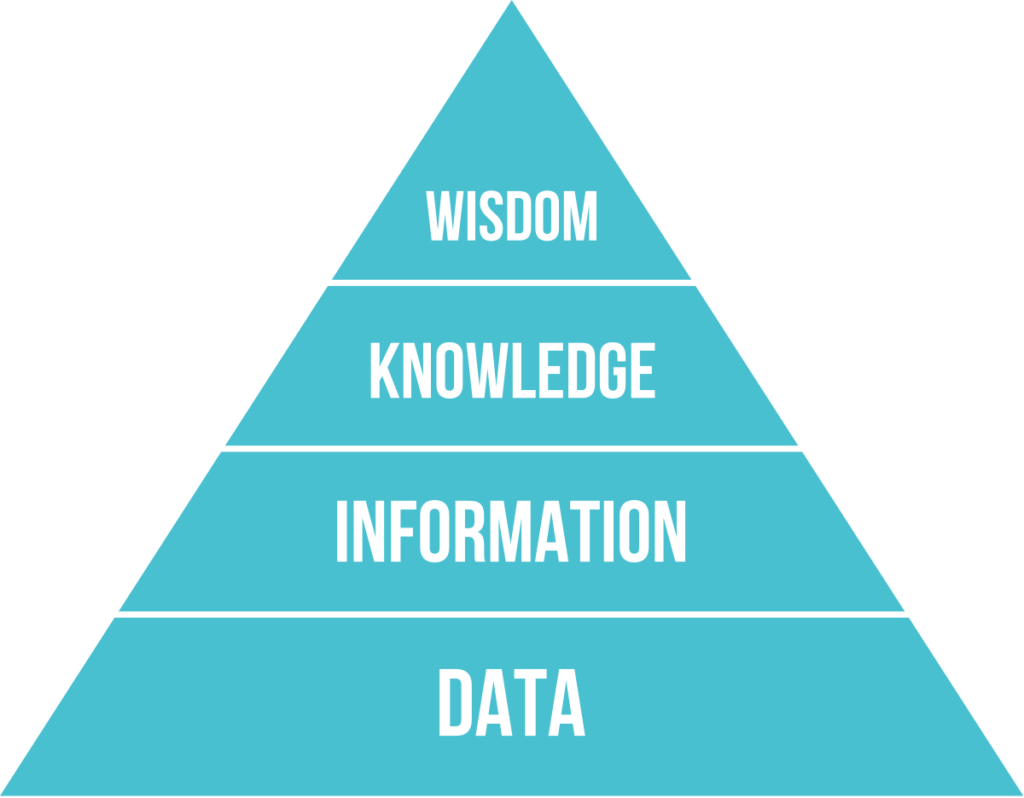
\includegraphics[scale=0.3]{PiramideDIKW}
\caption{Piramide DIKW. Fonte: \href{https://www.bigdata4innovation.it/big-data/la-piramide-dikw-cose-e-cosa-rappresenta/}{www.bigdata4innovation.it}}
\end{figure}

I \textbf{dati} sono rappresentati da stimoli o segnali e rimangono inutili fino a quando non vengono elaborati in qualche forma:
\begin{itemize}
\item \textit{universale}, quando sono prodotti dall'osservazione
\item \textit{soggettivi}, quando sono prodotti dagli stessi.
\end{itemize}
Inoltre possiamo definire diversi tipi di dato:
\begin{itemize}
\item \textit{fatti}, costituiti da osservazioni discrete, oggettive, non organizzate o elaborate, in assenza di un contesto interpretativo.
\item \textit{segnali}, presenti nel dominio soggettivo come letture di segnali e stimoli sensoriali.
\item \textit{simboli}, costituiti da insiemi di segni che rappresentano le percezioni di proprietà di oggetti, eventi o dell'ambiente.
\end{itemize}

Le \textbf{informazioni} sono rappresentate da dati dotati di significato o di scopo, ed è rappresentata da una descrizione distinta dai dati per la sua utilità. L'informazione viene infierita sui dati rendendoli utili a prendere determinate decisioni o rispondendo a determinate domande. Se i dati sono organizzati per conferire particolare importanza in determinati contesti o per farli risultare significativi e utili, si parla di \textit{informazione strutturale e informazione funzionale}. Se invece l'informazione è costituita da simboli o da segni, prende il nome di \textit{informazione universale}, mentre se ad essa si associa un significato al quale si collegano dei simboli, si parla di \textit{informazione soggettiva}.

Quando l'informazione viene elaborata, organizzata, o altrimenti applicata si parla di \textbf{conoscenza}, nella quale si ha anche una commistione di esperienza, valori e comprensione profonda. La conoscenza fornisce un ambiente e una struttura per la valutazione  e l'acquisizione di nuove esperienze e informazioni. Vi sono diversi tipi di conoscenza:
\begin{itemize}
\item \textbf{conoscenza elaborata}, definita come sintesi di più sorgenti fi informazioni nello stesso tempo.
\item \textbf{conoscenza procedurale},definita come applicazione di dati e informazioni raggiunte attraverso un'esperienza pratica.
\item \textit{conoscenza procedurale}, nella quale le credenze vengono strutturate in termini proposizionali o soggettivamente. 
\end{itemize}

Adesso siamo pronti a dare una definizione di \textbf{intelligenza artificiale} come la disciplina che mira a studiare e comprendere i principi che rendono possibile un comportamento intelligente in sistemi artificiali. Secondo Church - Turing è presente un livello di astrazione in cui si può interpretare il ragionamento come manipolazione di simboli e un livello artificiale come computazionale. Nella progettazione di sistemi intelligenti basati su conoscenza possiamo distinguere sostanzialmente tre fasi principali:
\begin{itemize}
\item \textit{fase di progetto}, svolta dal progettista, nella quale si conduce uno studio del progetto;
\item \textit{fase offline}, che precede l'osservazione del mondo e si base sull'apprendimento o compilazione della conoscenza, la comprensione della \textit{conoscenza di fondo (BK)} data o definita in precedenza, oppure si ricava una \textit{base di conoscenza (KB)} da utilizzare nelle fasi successive.
\item \textit{online}, fase nella quale si passa dalla decisione all'azione. Si ottengono informazioni dalle osservazioni e si prendono decisioni su azioni da svolgere usando la KB.
\end{itemize}

Si possono verificare due casi estremi, ovvero il caso in cui il sistema diventa specializzato nel suo dominio e inutile al di fuori di questo, e il caso in cui il sistema è flessibile, ovvero che si adatta ai vari casi d'uso. Un sistema può essere costruito semplificando il modello dell'ambiente costruendo sistemi di ragionamento complessi, facilitando così la dimostrazione di proprietà o l'ottimizzazione, oppure si costruiscono sistemi semplici per contesti complessi.

Nell'AI è molto importante distinguere il cosa vada calcolato dal come. Si deve formalizzare cosa costituisca una soluzione e rappresentare il problema in un linguaggio su cui il sistema possa ragionare. Successivamente si fa calcolare al sistema l'output e lo si interpreta come soluzione al problema.
Conoscere l'informazione sul dominio è utile a risolvere i problemi. Bisogna scegliere il linguaggio più utile a rappresentare le informazioni sul dominio utile a risolvere i problemi. La formalizzazione della conoscenza all'interno della macchina richiede il rispetto di alcune proprietà importanti, quali \textit{la ricchezza espressiva}, \textit{la vicinanza} ai termini del problema che permette di facilitare l'individualizzazione delle relazioni fra il dominio reale e la sua rappresentazione per verificarne la correttezza, \textit{l'efficienza} nella sua elaborazione, utilizzando quindi poche risorse, e deve essere \textit{acquisibile} dai dati e da esperienza pregressa.

Una proprietà importante dei linguaggi di rappresentazione è la loro capacità di essere estesi rispetto agli obiettivi principali per i quali sono stati concepiti. Per esempio i \textit{linguaggi per l'apprendimento} possono essere estesi per ammettere maggiori capacità risolutive o di inferenza, \text{i linguaggi espressivi} possono essere estesi per aggiungere capacità di inferenza e apprendimento, mentre \textit{i linguaggi semplici} utilizzati per dimostrare la trattabilità del calcolo, possono essere estesi in maniera più naturale per agevolare l'acquisizione di conoscenza.

Un argomento molto importante è la quantità di conoscenza da utilizzare. Per \textit{gli agenti umani}, viene richiesta una quantità di conoscenza molto elevata anche per compiti molto semplici, mentre per gli \textit{agenti software}, non è richiesta molta conoscenza e diventano sempre più bravi in compiti in cui la conoscenza di base intensiva e nei compiti in cui acquisiscono in autonomia conoscenza per compiti specifici.

La \textbf{soluzione} è costituita da un raffinamento della specifica del sistema, dall'automatizzazione di forme di senso comune, oppure da una soluzione che non è una soluzione generica ma specifica rispetto a un dato criterio. Si parla di \textit{soluzione ottimale} quando si deve cercare la migliore soluzione in base a una misura di qualità ordinale o cardinale. Una soluzione è una \textit{soluzione soddisfacente} quando si cerca una soluzione buona in base a una determinata descrizione, perchè quella migliore è troppo costosa da trovare. Se l'obiettivo è di trovare una soluzione di qualità prossima a quella teoricamente ottimale, si parla di una \textit{soluzione approssimata}. Infine se si cerca una soluzione verosimile con un certo grado di certezza, si parla di una \textit{soluzione probabile}.

Nella \textbf{rappresentazione} di un problema ci si chiede come acquisire e rappresentare la conoscenza su un dominio e di come usarla per rispondere a domande o risolvere dei problemi. Una soluzione a questo problema consiste nell'utilizzare la logica per specificare il significato, utilizzando anche notazioni come la sintassi del Datalog. Si possono usare \textbf{sistemi simbolici fisici} già conosciuti o crearne uno adatto al progetto che stiamo realizzando, definendo i \textit{simboli}, ovvero pattern significativi manipolabili come singole unità, e un \textit{sistema di simboli} che serve a creare, copiare, modificare e distruggere i simboli. 
In questo ambito è importante ricordarsi l'ipotesi di Newell e Simon, i quali sostenevano che un sistema di simboli ha i mezzi necessari e sufficienti per un'azione intelligente. Questa ipotesi ha delle conseguenze importanti a livello empirico. Un sistema intelligente è quindi un sistema simbolico fisico, ha tutto il necessario per un comportamento intelligente e non esclude l'uso di un corpo per percepire il mondo e agire su di esso. Un sistema quindi manipola simboli per produrre decisioni o azioni sui simboli che riferiscono ai vari oggetti del mondo e sugli altri simboli interni che potrebbero rimandare a concetti utili anche senza avere un significato per l'esterno. 

Lo scopo principale di un sistema di simboli è quello di modellare il mondo rappresentando ciò che deve essere considerato vero nel mondo o della sua dinamica. Si parla di astrazione quando il sistema non è troppo dettagliato e trascura quindi dei dettagli. Se vengono forniti maggiori dettagli rispetto a una semplice astrazione si parla di un ordine parziale, mentre il modello del mondo per eccellenza consiste nell'insieme di più modelli che lo descrivono anche se in contraddizione tra di loro e vengono giudicati in base alla loro utilità.

In base al \textbf{singolo livello di astrazione} si dividono descrizioni di \textit{alto livello} quando si descrivono i modelli in maniera comprensibile per gli umani, in maniera poco formale, mentre le descrizioni di \textit{basso livello} sono più accurate e dettagliate, essenziali per la soluzione del problema, mentre quelle di \textit{più basso livello}.

La \textbf{complessità} di un sistema è variabile e dipende dagli agenti e dai vari sistemi che compongono il sistema finale. Vi sono diverse dimensioni della complessità che vanno combinate anche se studiate separatamente, definiscono gli spazi di progettazione all'interno dei sistemi intelligenti e definiscono una decomposizione sommaria dello spazio di progettazione.

Il grado di decomposizione di un sistema in moduli interagenti prende il nome di \textbf{modularità}. Questa caratteristica è fondamentale per dominare la complessità di un sistema, decomponendolo gerarchicamente. Si identificano tre livelli possibili di strutture:
\begin{itemize}
\item \textbf{struttura piatta}, nella quale non vi è presente nessuna struttura organizzativa
\item \textbf{struttura modulare}, nella quale il sistema è decomposto in moduli interagenti che possono però essere considerati separatamente
\item \textbf{gerarchica}, nella quale i moduli sono decomposti in sotto moduli interagenti, decomponibili a loro volta in maniera gerarchica.
\end{itemize}
Nella modularità è di fondamentale importanza lo \textbf{schema di rappresentazione}, che descrive il mondo caratterizzandolo in stati distinti che hanno un impatto sul comportamento del sistema, descrivendo lo stato interno del sistema e lo stato dell'ambiente, e individuando stati identificati individualmente.
In ogni sistema conviene ragionare in termini di \textbf{caratteristiche} degli stati (feature) o proposizioni booleane. Nei mondi più complessi le caratteristiche dipendono dalle relazioni e dagli individui. Si definisce \textbf{proprietà} una relazione su un singolo individuo, invece si definisce una \textbf{caratteristica} per ogni possibile relazione tra gli individui.

A volte ci si trova a lavorare in uno stato di \textbf{incertezza} all'interno del dominio, considerando osservazioni e percezioni. In queste situazioni non sempre si può osservare direttamente lo stato del mondo, e a volte succede che ciò che si osserva consista in un'osservazione difettosa o parziale. Da qui deriva l'espressione \textbf{incertezza sulla percezione}, che riguarda la possibilità di determinare lo stato del mondo attraverso osservazioni. Si parla quindi di \textbf{stato pienamente osservabile}, quando esso può essere conosciuto dalle osservazioni, mentre si definisce \textbf{stato parzialmente osservabile}, quando non è osservato direttamente.

Anche gli effetti di azioni o decisioni possono essere predetti con certezza o in maniera incerta. In quest'ultimo caso si parla di \textbf{incertezza sugli effetti}, secondo la quale, la loro dinamica può essere \textit{deterministica}, quando lo stato risultante può essere determinato esattamente dall'azione e dallo stato precedente, o \textit{aleatoria} nella quale la probabilità sui possibili risultati ha senso se il mondo è completamente osservabile o altrimenti è stocastica, modellata come deterministica ma con effetti che dipendono da feature non osservate.

Gli agenti sono molto spesso \textit{utilitaristici}, quando essi scelgono un'azione in base ai risultati attesi o desiderabili, e possono avere finalità semplici o preferenze complesse. Le \textbf{preferenze} si caratterizzano come finalità da raggiungere (achievement goal) in uno stato finale o di conservazione (maintenance goal) in ogni stato visitato,  o come \textbf{preferenze complesse} rappresentate da 



\end{document}



